\documentclass{article}
\usepackage{graphicx} % Required for inserting images
\usepackage[sortcites=true]{biblatex}

\addbibresource{final.bib}
\title{Parallel Oblivious Sorting in SGX Enclave}
\author{Tianyao Gu, Tian Xie}
\date{December 2023}

\begin{document}

\maketitle

\begin{abstract}
    Oblivious algorithms have been a popular research topic in cybersecurity as it guarantees a simulatable memory access pattern and thereby provably resists side channel attacks. We implemented a parallel oblivious sorting algorithm in C++ using Intel SGX Enclave, a hardware-based trusted-computing environment offering privacy and authenticity. We leveraged OpenMP to achieve multithreading on a 36-core CPU, and further improves parallelism through SIMD. We increased the arithmetic density of the algorithm to make it efficient in an external memory model. We optimized the memory utilization of the program to minimize the consumption of Enclave Page Cache. We also overlapped computation and communication through prefetching and write back buffers.
\end{abstract}

\section{Background}
\subsection{Background on Oblivious Sorting Algorithms}
Our motivation is to securely outsource data and computation to an untrusted worker equipped with secure processors such as Intel SGX. Although secure processors ensure data privacy through encryption, existing literature reveals that attackers can exploit memory access and page swap patterns during computations to glean information about the data.

Oblivious algorithms provide a verifiable shield to counter such side-channel attacks. This is because ``Obliviousness'' essentially demands that memory access and page swap patterns remain independent of secret data. 

In addition, sorting stands out as a fundamental building block of various oblivious computation applications. Specifically, oblivious sorting is
key to common
graph algorithms~\cite{oblivm,blantongraph,oram09} including
breadth-first search~\cite{oram09,blantongraph},
connected components~\cite{domulticore},
minimum spanning tree/forest~\cite{domulticore},
clustering~\cite{oblivm},
list ranking~\cite{domulticore}, tree computations with Euler tour~\cite{domulticore},
and tree contraction~\cite{domulticore}.
Oblivious sorting can also be used for securely initializing
common ORAM algorithms~\cite{enigmap} including
Path ORAM~\cite{pathoramjrnl}, which has been deployed at a large scale
in practice~\cite{signalpathoram}.
Moreover, any computational task
that can be efficiently expressed as a streaming-Map-Reduce algorithm
has an efficient
oblivious implementation using oblivious sort~\cite{oram09,oblivm}.

Our project is based on a prior research paper by Gu et al.~\cite{osort}. The paper proposed and implemented an efficient oblivious sorting in hardware enclaves, which achieves asymptotically optimal runtime and outperforms all the previous works concretely. However, the algorithm, as presented and implemented, is single-threaded, posing limitations on its performance.

In our continuation of this work, we aim to enhance performance by parallelizing the oblivious sorting algorithm. As a byproduct, we obtain a parallel oblivious random shuffling algorithm, which is also a crucial primitive in oblivious computation.

\subsection{Background on Flex-way Butterfly Oblivious Sort}
To achieve oblivious sorting, Asharov et al.~\cite{bucketsort} proposed the idea to first design an {\it oblivious random bucket assignment}
algorithm, which randomly assigns each
input element to one of $O(N/Z)$ output buckets, each of poly-logarithmic
capacity $Z$; further, the obliviousness property requires that
the access patterns do not leak the destination bucket of each element.
Then, from the oblivious random bucket assignment, they
get an {\it oblivious shuffling} algorithm,
which randomly permutes
the inputs without revealing the permutation. Finally,
they can apply any non-oblivious, comparison-based sorting algorithm to the shuffled array.

Flex-way Butterfly Oblivious Sort~\cite{osort} adopts this idea and achieved the {\it oblivious random bucket assignment} using a multi-way butterfly network. The input of the network consists of $(1+\epsilon)N/Z$ buckets of size $Z$, where each bucket contains $Z/(1+\epsilon)$ real input elements and is padded with filler elements. Each element is attached a random tag.

The network relies on an important building block called multi-way {\sf MergeSplit}, which merges elements from $k$ buckets and obliviously splits the real elements into $k$ buckets according to the modulus of their tags. Because each bucket is padded with filler elements, the no bucket will overflow except with negligible probability. Figure \ref{fig:butterfly} demonstrates a 3-level butterfly network that assigns elements to 18 buckets.

\begin{figure}[thbp]
    \centering
    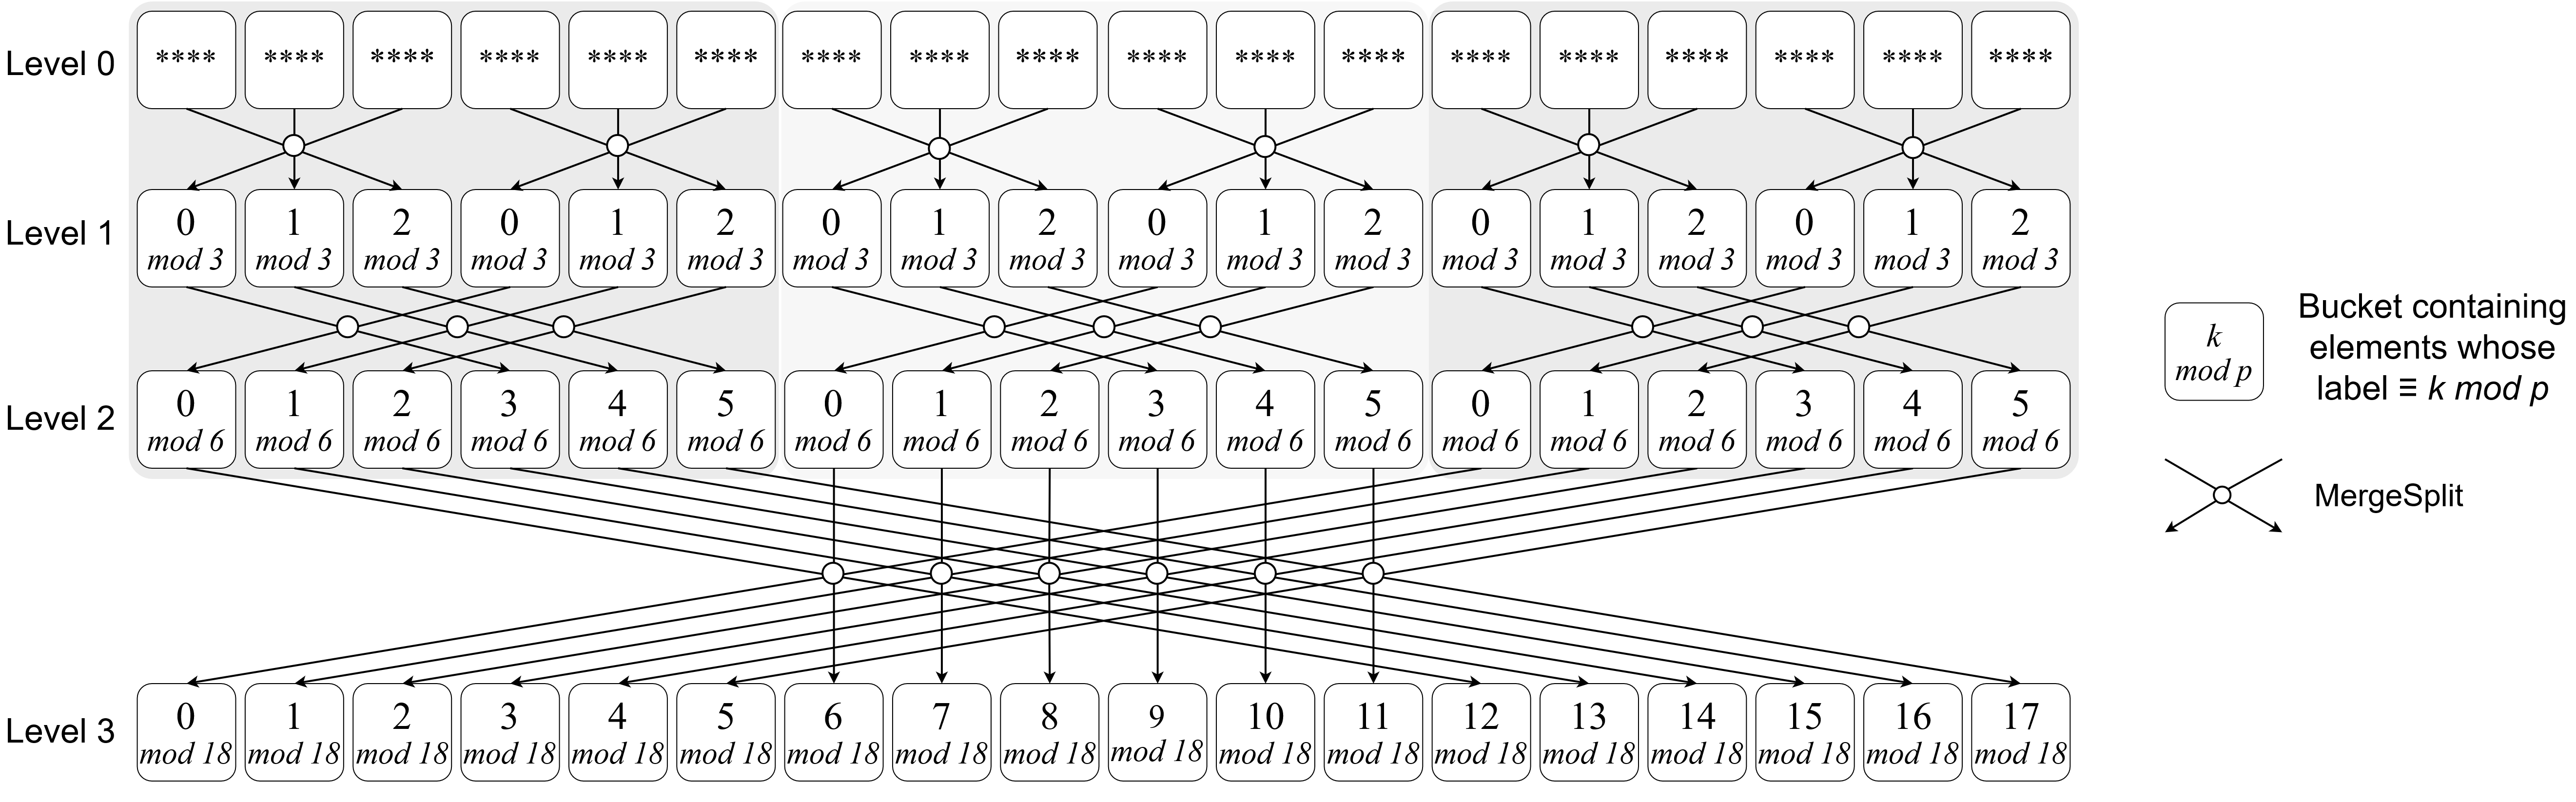
\includegraphics[width=\textwidth]{assets/multi-way-butterfly.png}
    \caption{A 3-level multi-way butterfly network.}
    \label{fig:butterfly}
\end{figure}


When implementing the algorithm in Intel SGX, we need to consider the memory limitations of the SGX enclave. When transferring data across the boundary of the enclave, we must pay an expensive cost for encryption, decryption, and authentication. Naively emulating the butterfly network level by level would incur an extra I/O overhead of $\Theta(\log N)$. Therefore, we want to route elements through multiple levels each time we fetch them into the enclave, as is demonstrated in Figure \ref{fig:batch}. This optimization significantly increases the arithmetic density of the algorithm and thereby improves performance.

\begin{figure}[thbp]
    \centering
    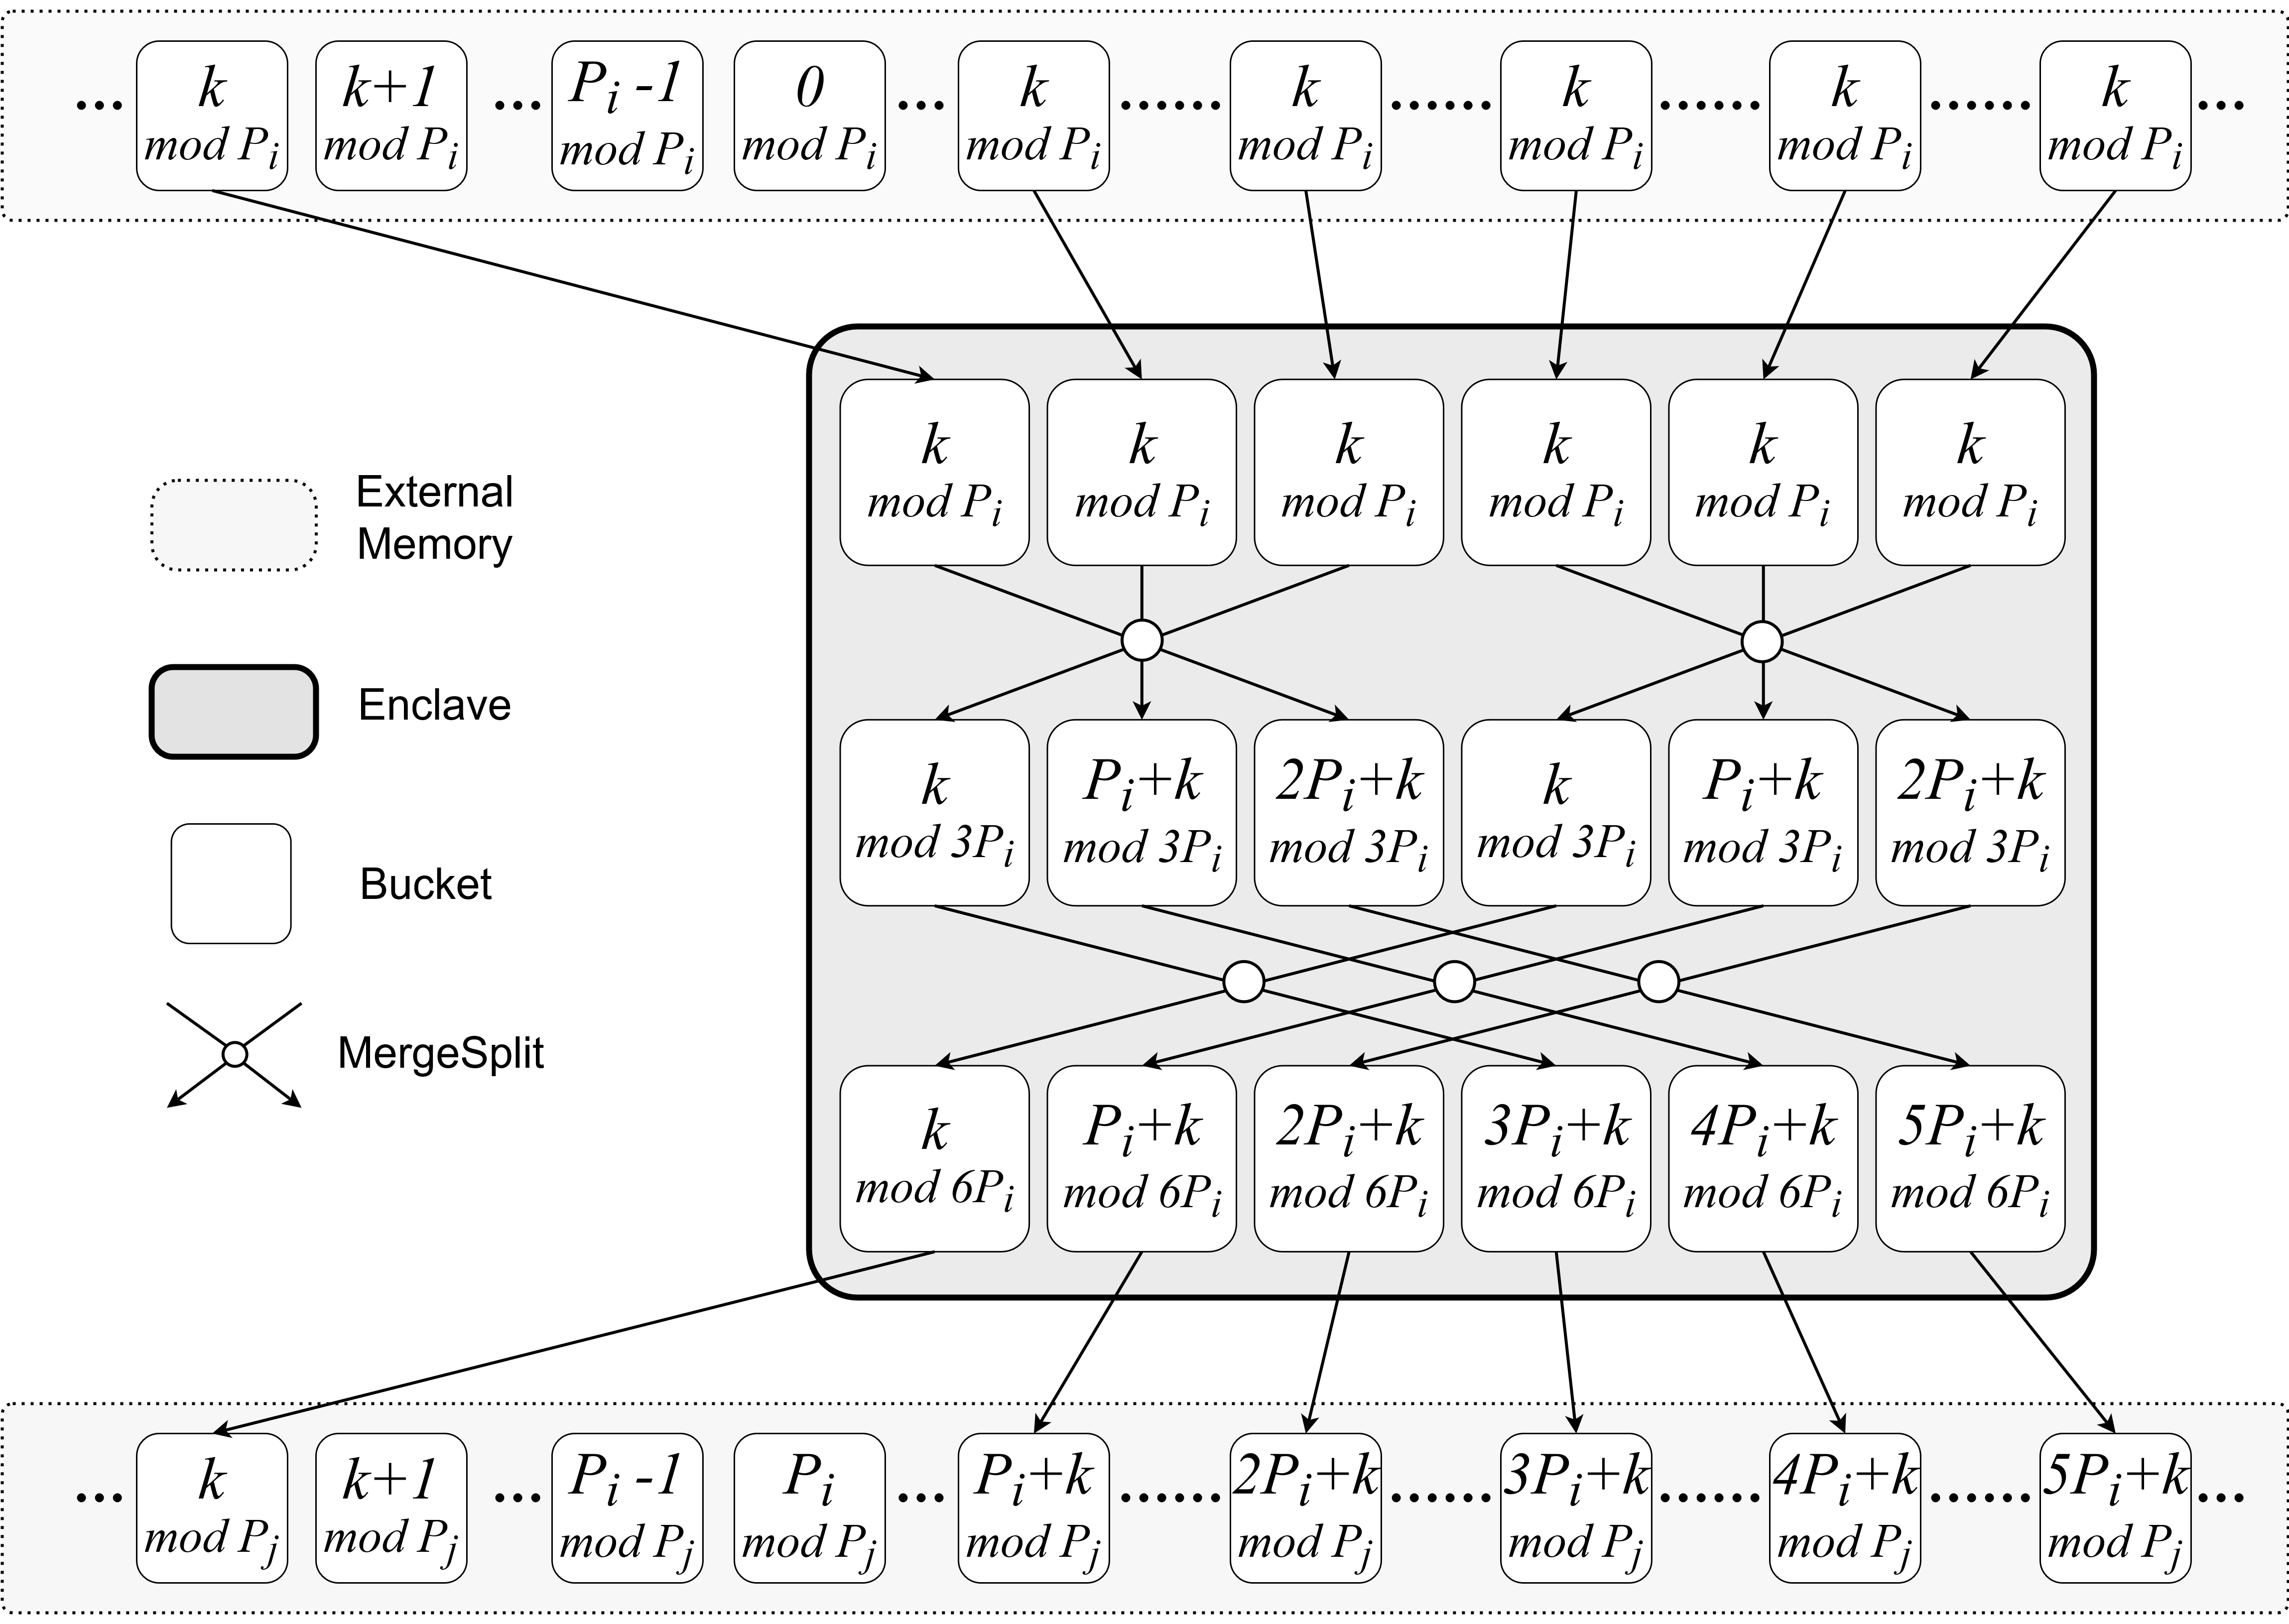
\includegraphics[width=0.8\textwidth]{assets/batch.png}
    \caption{Route elements through multiple levels of butterfly network in each batch.}
    \label{fig:batch}
\end{figure}



\section{Approach}
\subsection{Identify Parallelism}

% We have successfully parallelized the oblivious shuffling algorithm in Intel SGX using OpenMP and SIMD.
% Specifically, our key accomplishments include:

% 1. Configured `OpenMP` in the Makefile and set up the multi-threaded environment in the SGX config files.

% 2. Changed the butterfly routing from recursion to iterative, which reduces the overhead of parallel execution. Also, we combined multiple batches into one batch when there's enough memory to increase parallelism.

% 3. Improved the parameter solver to ensure that there are enough parallel tasks on each butterfly network level (by reducing bucket size and balancing the mergesplit ways on each level.)

% 4. Applied `#omp parallel for` to parallelize the butterfly network executions.

% 5. Applied `#omp parallel for` to parallelize I/O operations with external memory.

% 6. Developed a reader/writer pool manager to fetch input and combine the final output, thereby reducing thread contention.

% 7. Separated a central pseudo-random number generator (which uses AES counter mode) to multiple ones to reduce contention.

% 8. Utilized C++ intrinsics to accelerate element-wise oblivious exchange using SIMD. Incorporated different instruction sets such as AVX512, AVX2, and SSE2 for broader processor compatibility.

% 9. Established unit tests on the algorithm outside the enclave for debugging and tuning. Installed Intel vtune software.


\section{Results}
\end{document}